\documentclass[border=10pt]{standalone}
\usepackage{pgfplots}
\pgfplotsset{width=7cm,compat=1.8}
\usetikzlibrary{spy}
\begin{document}
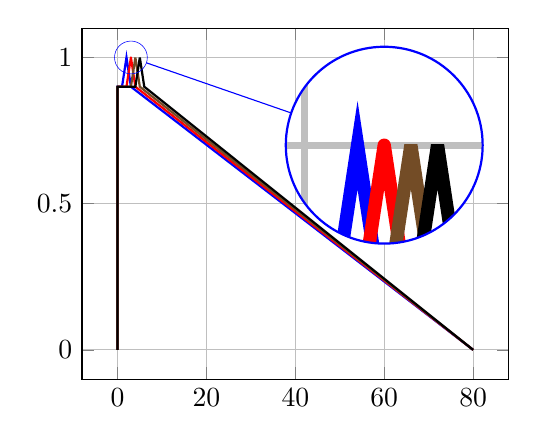
\begin{tikzpicture}[spy using outlines=
	{circle, magnification=6, connect spies}]
\begin{axis}[no markers,grid=major,
	every axis plot post/.append style={thick}]
\addplot  coordinates
 {(0, 0.0) (0, 0.9) (1, 0.9) (2, 1) (3, 0.9) (80, 0)};
\addplot +[line join=round] coordinates
 {(0, 0.0) (0, 0.9) (2, 0.9) (3, 1) (4, 0.9) (80, 0)};
\addplot +[line join=bevel] coordinates
 {(0, 0.0) (0, 0.9) (3, 0.9) (4, 1) (5, 0.9) (80, 0)};
\addplot +[miter limit=5] coordinates
 {(0, 0.0) (0, 0.9) (4, 0.9) (5, 1) (6, 0.9) (80, 0)};

  \coordinate (spypoint) at (axis cs:3,1);
  \coordinate (magnifyglass) at (axis cs:60,0.7);
\end{axis}

\spy [blue, size=2.5cm] on (spypoint)
   in node[fill=white] at (magnifyglass);
\end{tikzpicture}
\end{document}